\chapter{Φυσικοί αριθμοί}

\section{Οι αριθμοί και η Python}

Οι φυσικοί αριθμοί είναι οι αριθμοί από 0, 1, 2, 3, 4, 5, 6, \ldots, 98, 99, 100, \ldots, 1999, 2000, 2001, \ldots

Η Python μπορεί να χειριστεί φυσικούς αριθμούς. Δοκιμάστε να γράψετε στο REPL έναν φυσικό αριθμό, θα δείτε ότι η Python θα τον επαναλάβει. Π.χ. δείτε τον αριθμό εκατόν είκοσι τρια (123).
\begin{lstlisting}
>>> 123
123
\end{lstlisting}

Στην Python όμως θα πρέπει να ακολουθείς κάποιους επιπλέον κανόνες. Για παράδειγμα στους αριθμούς δεν πρέπει να βάζεις τελείες στις χιλιάδες όπως στο χαρτί. Αν το κάνεις στην καλύτερη περίπτωση θα προκύψει κάποιο λάθος, στην χειρότερη ο υπολογιστής θα καταλάβει διαφορετικό αριθμό από αυτόν που εννοείς.
Δείτε το παρακάτω παράδειγμα στο REPL.
\begin{lstlisting}
>>> 1.000.000
  File "<stdin>", line 1
    1.000.000
            ^
SyntaxError: invalid syntax
>>> 100.000
100.0
\end{lstlisting}
Σε αυτό το παράδειγμα, η Python δεν καταλαβαίνει καθόλου τον αριθμό 1.000.000 γραμμένο με τελείες ενώ μεταφράζει το 100.000 σε 100.0, που για την Python σημαίνει 100 (εκατό). Γι' αυτόν τον λόγο δεν βάζουμε καθόλου τελείες έτσι αν θέλουμε να γράψουμε το ένα εκατομμύριο θα γράψουμε 1000000.
\begin{lstlisting}
>>> 1000000
1000000
\end{lstlisting}

\section{Πρόσθεση, αφαίρεση και πολλαπλασιασμός φυσικών αριθμών}
Μια γλώσσα προγραμματισμού μπορεί να εκτελέσει απλές πράξεις πολύ εύκολα. Στο βιβλίο των μαθηματικών  σου μπορείς να βρεις πολλές ασκήσεις με πράξεις. Μπορείς να τις λύσεις με την Python.

\begin{exercise}
\sel{16}
Να υπολογιστούν τα γινόμενα: 

(α) $35 \cdot 10$, 

(β) $421 \cdot 100$,

(γ) $5 \cdot 1.000$,

(δ) $27 \cdot 10.000$
\end{exercise}

Η python μπορεί να κάνει αυτές τις πράξεις ως εξής:
\begin{lstlisting}
>>> 35*10
350
>>> 421*100
42100
>>> 5*1000
5000
>>> 27*10000
270000
\end{lstlisting}

Ο τελεστής του πολλαπλασιασμού είναι το αστεράκι * (SHIFT+8) στο πληκτρολόγιο. Εναλλακτικά, μπορείτε να το βρείτε στο αριθμητικό πληκτρολόγιο. 

\begin{exercise}
\sel{16}
Να εκτελεστούν οι ακόλουθες πράξεις:

(α) $89\cdot 7 + 89\cdot 3$

(β) $23 \cdot 49 + 77 \cdot 49$

(γ) $76 \cdot 13 – 76 \cdot 3$

(δ) $284 \cdot 99$
\end{exercise}
\begin{lstlisting}
>>> 89*7+89*3
890
>>> 23*49+77*49
4900
>>> 76*13-76*3
760
>>> 284*99
28116
\end{lstlisting}

Στις παραπάνω περιπτώσεις η python εκτελεί πρώτα τους πολλαπλασιασμούς και μετά τις προσθέσεις/αφαιρέσεις δίνοντας έτσι το αποτέλεσμα που αναμένεται. Για παράδειγμα 89\*7 + 89\*3 = 623 + 267 = 890, που είναι το σωστό αποτέλεσμα.

\begin{exercise}
\sel{18}
Υπολογίστε:

(α)  $157 + 33$ 

(β)  $122 + 25 + 78$

(γ)  $785 - 323$

(δ)  $7.321 - 4.595$

(ε)  $60 - (18 - 2)$

(στ) $52 - 11 -9$

(ζ)  $23 \cdot 10$

(η)  $97 \cdot 100$

(θ)  $879 \cdot 1.000$
\end{exercise}
Σε python τα παραπάνω υπολογίζονται ως εξής:
\begin{lstlisting}
>>> 157+33
190
>>> 122+25+78
225
>>> 785-323
462
>>> 7321-4595
2726
>>> 60-(18-2)
44
>>> 52-11-9
32
>>> 23*10
230
>>> 97*100
9700
>>> 879*1000
879000
\end{lstlisting}
Οι παρενθέσεις (SHIFT+9 και SHIFT+0) αλλάζουν τη σειρά των πράξεων. Οι πράξεις που είναι μέσα στην παρένθεση εκτελούνται πρώτες. Γι' αυτό το λόγο 60-(18-2)=60-16=44.

\begin{exercise}
\sel{18}
Σε ένα αρτοποιείο έφτιαξαν μία μέρα 120 κιλά άσπρο ψωμί, 135 κιλά χωριάτικο, 25 κιλά σικάλεως και 38 κιλά πολύσπορο. Πουλήθηκαν 107 κιλά άσπρο ψωμί, 112 κιλά χωριάτικο, 19 κιλά σικάλεως και 23 κιλά πολύσπορο. Πόσα κιλά ψωμί έμειναν απούλητα;
\end{exercise}
Με τις γνώσεις που έχουμε θα πρέπει να μετατρέψουμε το παραπάνω πρόβλημα σε μια αριθμητική παράσταση ώστε η python να μπορεί να την υπολογίσει, στη συγκεκριμένη περίπτωση η σωστή παράσταση είναι $$(120-107)+(135-112)+(25-19)+(38-23)$$
\begin{lstlisting}
>>> (120-107)+(135-112)+(25-19)+(38-23)
57
\end{lstlisting}
και η απάντηση είναι 57 κιλά ψωμί.

\section{Δυνάμεις φυσικών αριθμών}
Ο τελεστής της python για τις δυνάμεις είναι ο **  (δυο φορές το αστεράκι). Δηλαδή, αν θέλουμε να υπολογίσουμε το $10^2$ θα γράψουμε 10**2, με όμοιο τρόπο μπορούμε να υπολογίσουμε και τις υπόλοιπες δυνάμεις. Δοκίμασε τα παρακάτω στο REPL.
\begin{lstlisting}
>>> 10**2
100
>>> 10**3
1000
>>> 10**4
10000
>>> 10**5
100000
>>> 10**6
1000000
\end{lstlisting}
Στη προτεραιότητα των πράξεων, οι δυνάμεις έχουν μεγλύτερη προτεραιότητα από τον πολλαπλασιασμό και την πρόσθεση. Οπότε όταν έχουμε και δυνάμεις σε μια παράσταση πρώτα γίνονται οι πράξεις στις παρενθέσεις, μετά οι δυνάμεις και μετά οι πολλαπλασιασμοί και οι προσθέσεις.
\begin{exercise}
\sel{21}
Να εκτελεστούν οι πράξεις 

 1. $(2\cdot 5)^4+4\cdot (3+2)^2$

 2. $(2+3)^3 - 8\cdot 3^2$

\end{exercise}
Οι αντίστοιχες εκφράσεις είναι (2*5)**4+4*(3+2)**2 και (2+3)**3 - 8*3**2.

\begin{lstlisting}
>>> (2*5)**4+4*(3+2)**2
10100
>>> (2+3)**3 - 8*3**2
53
\end{lstlisting}
H 8*3**2 υπολογίζεται ως $8\cdot (3^2)$, δηλαδή $8\cdot 9 = 72$, αφού πρώτα γίνεται η δύναμη και μετά οι πολλαπλασιασμοί.

\begin{exercise}
Κάνε τις πράξεις: 
(α) $3\cdot 5^2$, 

(β) $3\cdot 5^2 + 2$, 

(γ) $3\cdot5^2 + 2^2$, 

(δ) $3\cdot 5 + 2^2$, 

(ε) $3\cdot(5 + 2)^2$.
\end{exercise}

Αυτές οι πράξεις μπορούν να γίνουν στο REPL.
\begin{lstlisting}
>>> 3*5**2
75
>>> 3*5**2 + 2
77
>>> 3*5**2 + 2**2
79
>>> 3*5 +2**2
19
>>> 3*(5 + 2)**2
147
\end{lstlisting}

\begin{exercise}
Κάνε τις πράξεις: 
(α) $3^2 +3^3 +2^3 +2^4$, 

(β) $(13-2)^ 4 + 5\cdot 3^2$
\end{exercise}

\begin{lstlisting}
>>> 3**2 +3**3 +2**3 +2**4
60
>>> (13-2)**4 + 5*3**2
14686
\end{lstlisting}

\begin{exercise}
Βρες τις τιμές των παραστάσεων: 

(α) $(6+5)^2$ και $6^2+5^2$, 

(β) $(3+6)^2$ και $3^2+6^2$.
\end{exercise}
\begin{lstlisting}
>>> (6+5)**2
121
>>> 6**2+5**2
61
>>> (3+6)**2
81
>>> 3**2+6**2
45
\end{lstlisting}


\section{Συγκρίσεις φυσικών αριθμών}
Μπορούμε να συγκρίνουμε αριθμούς στην Python χρησιμοποιώντας τους τελεστές == (πληκτρολογούμε δύο φορές το =) για την \emph{ισότητα}, > για το \emph{μεγαλύτερο} και < για το \emph{μικρότερο}. Επίσης μπορούμε να χρησιμοποιήσουμε >= για το \emph{μεγαλύτερο ή ίσο} και <= για το \emph{μικρότερο ή ίσο}, τέλος υπάρχει το != για το \emph{δεν είναι ίσο}. Μπορείς να δοκιμάσεις τα παρακάτω:
\begin{lstlisting}
>>> 123==123
True
>>> 123>123
False
>>> 123>122
True
>>> 123<123
False
>>> 123<124
True
>>> 123<=123
True
>>> 123<=124
True
>>> 123<=122
False
>>> 123>=123
True
>>> 123>=124
False
>>> 123>=122
True
>>> 122 != 123
True
>>> 122 != 122
False
\end{lstlisting}
Η Python επιστρέφει True (αληθές) όταν μία πρόταση ισχύει και False (ψευδές) όταν δεν ισχύει.

Σκέψου ότι για την Python η σύγκριση είναι και αυτή μια πράξη. Αντί η πράξη αυτή να δίνει σαν αποτέλεσμα έναν αριθμό δίνει σαν αποτέλεσμα το αληθές ή το ψευδές.

Για παράδειγμα:
\begin{exercise}
Να συγκρίνετε τα $3^2$ και $2^3$.
\end{exercise}
Η σύγκριση αυτή μπορεί να γίνει στο REPL. Δοκίμασε:
\begin{lstlisting}
>>> 3**2 > 2**3
True
\end{lstlisting}
Άρα το $3^2$ είναι μεγαλύτερο από το $2^3$. Θυμήσου ότι το $3^2=9$, ενώ $2^3=8$.
\begin{exercise}
\end{exercise}

\section{Η εντολή print}
Ήρθε η ώρα να γράψεις εντολές στο πάνω παράθυρο, δηλαδή να γράψεις το πρώτο σου πρόγραμμα.  Με βάση όσα ξέρεις προσπάθησε να γράψεις μια πράξη στο πάνω παράθυρο, για παράδειγμα $32+35$. Ύστερα πάτησε το κουμπί της εκτέλεσης (Run). Μπορείς να δεις το αποτέλεσμα στην εικόνα \ref{noprint}.
\begin{figure}
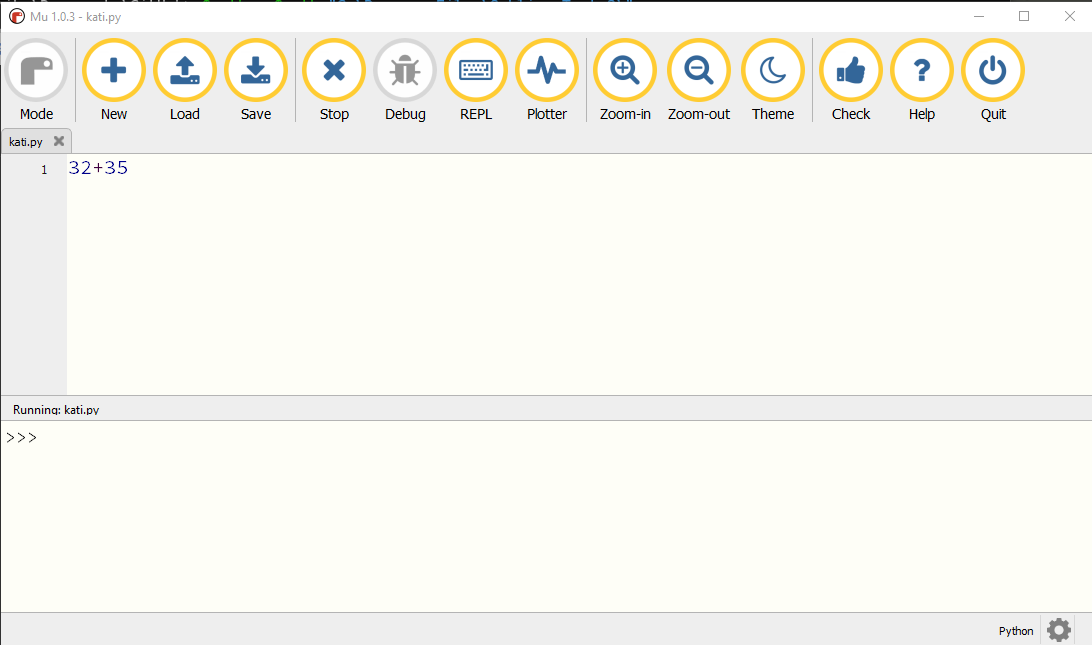
\includegraphics[width=\textwidth]{noprint.png}
\caption{Η εκτέλεση δεν δίνει κάποιο αποτέλεσμα}
\label{noprint}
\end{figure}

Η Python εκτελεί την πράξη $32+35$, και υπολογίζει το αποτέλεσμα. Αν δεν το έκανε και υπήρχε κάποιο πρόβλημα θα εμφάνιζε κάποιο μήνυμα λάθους στο REPL. Το υπολογισμένο αποτέλεσμα δεν εμφανίζεται. Για να εμφανιστεί το αποτέλεσμα πρέπει να χρησιμοποιήσεις την εντολή print (εκτύπωσε). Η εντολή print εκτελείται ως εξής:
\begin{lstlisting}
print(32+35)
\end{lstlisting}
Γράφουμε δηλαδή, print ανοίγουμε παρένθεση, γράφουμε αυτό που θέλουμε να εκτυπωθεί και κλείνουμε την παρένθεση. Όταν εκτελέσουμε το πρόγραμμα με την print τότε εμφανίζεται το αποτέλεσμα στο REPL (εικόνα \ref{withprint}).
\begin{figure}
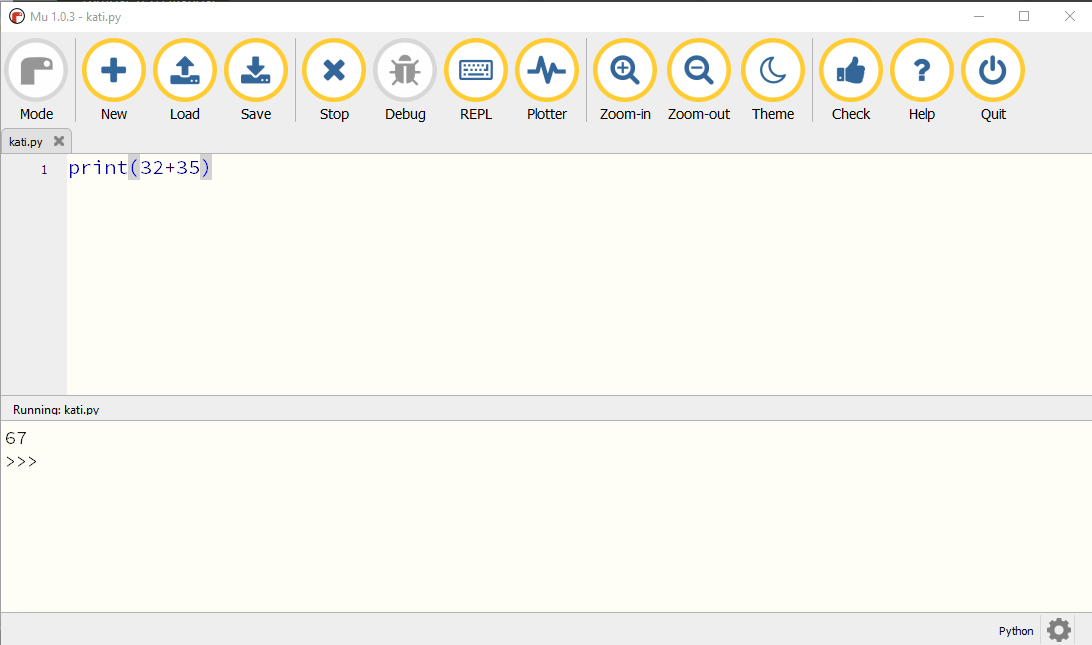
\includegraphics[width=\textwidth]{withprint.png}
\caption{Η εκτέλεση δίνει το αποτέλεσμα της πράξης}
\label{withprint}
\end{figure}
Μόλις έγραψες το πρώτο σου πρόγραμμα στην Python. Μάλιστα το πρόγραμμά σου κάνει κάτι. Υπολογίζει το αποτέλεσμα της πράξης $32+35$.
Μπορείς να αποθηκεύσεις το πρόγραμμά σου στον υπολογιστή σου κάνοντας κλικ στο εικονίδιο Save του Mu (εικόνα \ref{savewithmu}).
\begin{figure}
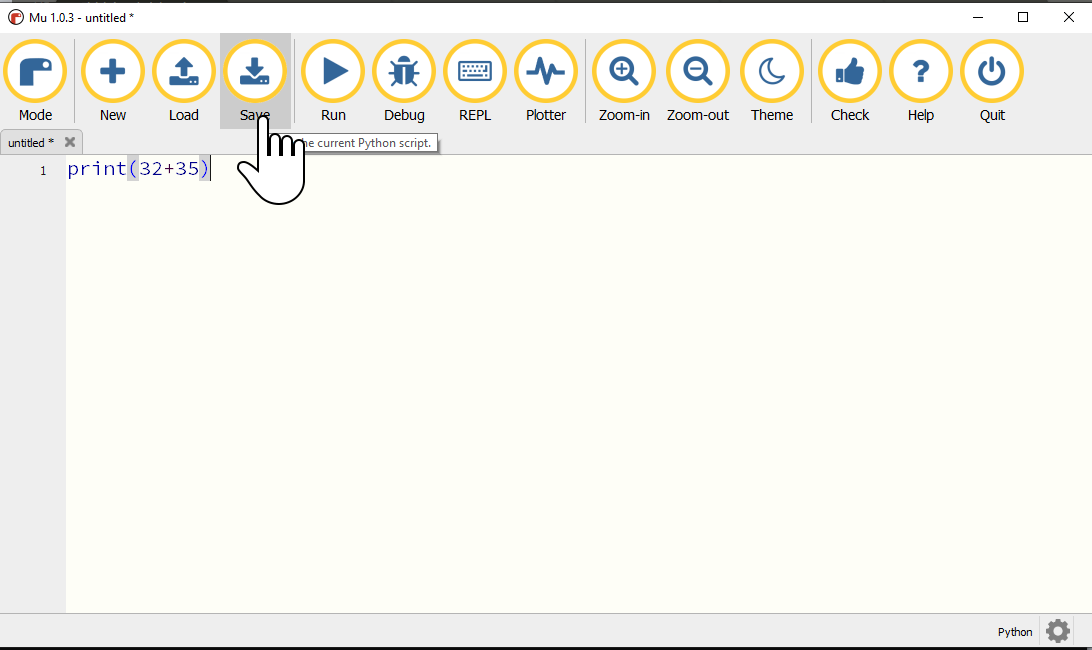
\includegraphics[width=\textwidth]{save.png}
\caption{Αποθήκευση με το Mu}
\label{savewithmu}
\end{figure}

\section{Απαρίθμηση}
Είδαμε ότι η Python μπορεί να κάνει πολύ γρήγορα, πολύπλοκες πράξεις ακόμη και με δυνάμεις, αλλά δεν είδαμε ακόμη τις απλές ασκήσεις που υπάρχουν στις πρώτες σελίδες του βιβλίου. Όπως για παράδειγμα ποιοι είναι οι τρεις προηγούμενοι αριθμοί του 289 και ποιο οι δύο επόμενοι (\sel{13}).

Τώρα που μάθαμε να γράφουμε προγράμματα σε Python μπορούμε να αντιμετωπίσουμε αυτό το πρόβλημα με το παρακάτω πρόγραμμα:
\begin{lstlisting}
print(289-3)
print(289-2)
print(289-1)
print(289+1)
print(289+2)
\end{lstlisting}
που δίνει το αποτέλεσμα
\begin{lstlisting}
286
287
288
290
291
\end{lstlisting}

Πιο σωστό θα ήταν να γράψουμε ποιοι αριθμοί είναι οι προηγούμενοι και ποιοι οι επόμενοι. Σε αυτή την περίπτωση θα γράψουμε τις παρακάτω εντολές.
\begin{lstlisting}
print("Οι  προηγούμενοι αριθμοί είναι:")
print(289-3)
print(289-2)
print(289-1)
print("Οι επόμενοι αριθμοί είναι:")
print(289+1)
print(289+2)
\end{lstlisting}

Για να εμφανίσει η print τις λέξεις που θέλουμε πρέπει να τις βάλουμε μέσα σε εισαγωγικά. Η Python υποστηρίζει είτε μονά εισαγωγικά, είτε διπλά. Αυτά εισάγονται συνήθως με το ίδιο κουμπί του πληκτρολογίου (κοντά στο ENTER), είτε με SHIFT ή χωρίς. Θυμήσου να κλείνεις τα εισαγωγικά με τον ίδιο τρόπο που τα άνοιξες. Στο πρόγραμμα Mu τα εισαγωγικά αυτά δεν φαίνονται όπως σε άλλα πρόγραμματα σαν `Εισαγωγικά' ή ``Εισαγωγικά " ή <<Εισαγωγικά>>, αλλά φαίνονται κάπως πιο απλά και ίδια στο άνοιγμα και το κλείσιμο \lstinline{'Εισαγωγικά'} ή  \lstinline{"Εισαγωγικά"}. 

Αν θέλουμε να αλλάξουμε το 289 και να βάλουμε έναν άλλο αριθμό,π.χ. το 132 θα πρέπει να αντικαταστήσουμε το 289 μέσα σε όλες τις εντολές print με το 132.
\begin{lstlisting}
print("Οι προηγούμενοι αριθμοί είναι:")
print(132-3)
print(132-2)
print(132-1)
print("Οι επόμενοι αριθμοί είναι:")
print(132+1)
print(132+2)
\end{lstlisting}

Υπάρχει όμως ένας καλύτερος τρόπος, ο τρόπος αυτός είναι να δώσουμε ένα όνομα στον αριθμό μας. Μπορούμε να πούμε ότι το n είναι το όνομα του αριθμού. Αυτό γίνεται με την εντολή \lstinline{n=132}. Τότε το πρόγραμμά μας γίνεται:
\begin{lstlisting}
n = 132
print("Οι προηγούμενοι αριθμοί είναι:")
print(n-3)
print(n-2)
print(n-1)
print("Οι επόμενοι αριθμοί είναι:")
print(n+1)
print(n+2)
\end{lstlisting}

Μετά την εντολή \lstinline{n=132} η Python ξέρει ότι το n είναι ένα όνομα για το 132 και μπορεί να κάνει πράξεις με αυτό. Για παράδειγμα n+1 κάνει τώρα 133.

Αν θέλουμε να κάνουμε τώρα το ίδιο πρόγραμμα αλλά όχι για το 132 αλλά για το 210, χρειάζεται να αλλάξουμε μόνο μία γραμμή και το πρόγραμμά μας να γίνει ως εξής:
\begin{lstlisting}
n = 210
print("Οι προηγούμενοι αριθμοί είναι:")
print(n-3)
print(n-2)
print(n-1)
print("Οι επόμενοι αριθμοί είναι:")
print(n+1)
print(n+2)
\end{lstlisting}

Στην Python, όταν δίνουμε ένα όνομα σε έναν αριθμό (με τον τελεστή =) τότε δημιουργούμε μια μεταβλητή. Η μεταβλητή έχει ένα όνομα, στην περίπτωσή μας το n, και μια τιμή, στην περίπτωσή μας το 210.

Αν αντί για τους επόμενους δύο αριθμούς θέλαμε τους επόμενους \textbf{δέκα} θα γράφαμε ένα πρόγραμμα όπως το παρακάτω:
\begin{lstlisting}
n = 210
print(n)
print(n+1)
print(n+2)
print(n+3)
print(n+4)
print(n+5)
print(n+6)
print(n+7)
print(n+8)
print(n+9)
print(n+10)
\end{lstlisting}
Το παραπάνω πρόγραμμα εμφανίζει και τον αριθμό μας n, δηλαδή το 210.

Για να μην γράφουμε πολλές εντολές όταν κάνουμε το ίδιο πράγμα χρησιμοποιούμε την εντολή for.
Το πρόγραμμά μας με την for μπορεί να γίνει:
\begin{lstlisting}
n = 210
for i in 0,1,2,3,4,5,6,7,8,9,10:
    print(n+i)
\end{lstlisting}
Όταν γράψεις την for στην Python θα πρέπει να δηλώσεις ποιες εντολές θα εκτελεστούν πολλές φορές. Αυτή η δήλωση γίνεται βάζοντας αυτές τις εντολές λίγο πιο μέσα χρησιμοποιώντας το πλήκτρο κενό ή το πλήκτρο tab. Μια καλή πρακτική είναι να βάζεις τέσσερα κενά. Έτσι, πριν την εντολή \lstinline{print(n+i)} βάζεις τέσσερα κενά δηλαδή \lstinline[showspaces=true]{    print(n+i)}.
Το πρόγραμμα αυτό σημαίνει πως για το i μέσα στο σύνολο 0, 1, 2, 3, \ldots 10 και με αυτή τη σειρά εμφάνισε το n+i. Έτσι το αποτέλεσμα είναι το αναμενόμενο
\begin{lstlisting}
210
211
212
213
214
215
216
217
218
219
220
\end{lstlisting}

Στην Python υπάρχει ένας πιο εύκολος τρόπος να γράψουμε τους αριθμούς από το 0 έως το 10. Αυτός ο τρόπος είναι η εντολή range και συγκεκριμένα η range(11). Η range(11) φτιάχνει τους αριθμούς από το 0 μέχρι το 10 οι οποίοι είναι σε πλήθος 11. 
Έτσι το πρόγραμμά μας γίνεται:
\begin{lstlisting}
n = 210
for i in range(11):
    print(n+i)
\end{lstlisting}

Mπορούμε και να μετρήσουμε τους πρώτους 100 αριθμούς ως εξής:
\begin{lstlisting}
n = 210
for i in range(100):
    print(n+i)
\end{lstlisting}

Σκέψου αν θα δεις τον αριθμό 100 στο αποτέλεσμα του παραπάνω προγράμματος.

\section{Στρογγυλοποίηση}
Το βιβλίο των Μαθηματικών της Α' Γυμνασίου αναφέρει πως
Για να στρογγυλοποιήσουμε έναν φυσικό αριθμό \sel{12}:
\begin{enumerate}
	\item Προσδιορίζουμε την τάξη στην οποία θα γίνει η στρογγυλοποίηση
	\item Εξετάζουμε το ψηφίο της αμέσως μικρότερης τάξης
	\item Αν αυτό το ψηφίο είναι μικρότερο του 5 (δηλαδή 0, 1, 2, 3 ή 4) το ψηφίο αυτό και όλα τα ψηφία των υπόλοιπων τάξεων μηδενίζονται.
	\item Αν είναι μεγαλύτερο ή ίσο του 5 (δηλαδή 5, 6, 7, 8 ή 9) το ψηφίο αυτό και όλα τα ψηφία των υπόλοιπων τάξεων αντικαθίστανται από το 0 και το ψηφίο της τάξης στρογγυλοποίησης αυξάνεται κατά 1.
\end{enumerate}

Ας πούμε ότι θέλουμε να στρογγυλοποιήσουμε τον αριθμό 454.018.512 στα εκατομμύρια. Η απάντηση που περιμένουμε είναι 454 εκατομμύρια.
Για να τα καταφέρουμε θα χρησιμοποιήσουμε την διαίρεση. Όμως στην Python υπάρχουν \emph{δύο} διαιρέσεις μία με το σύμβολο / και μία με το σύμβολο //. Ας δούμε τις διαφορές τους στο REPL.
\begin{lstlisting}
>>> x = 454018512
>>> print(x/1000000)
454.018512
>>> print(x//1000000)
454
\end{lstlisting}
Η <<κανονική>> διαίρεση, με τη μία κάθετο /, δίνει το αποτέλεσμα της διαίρεσης με τα δεκαδικά ψηφία. Η <<ακέραια>> διαίρεση δίνει μόνο τον ακέραιο αριθμό. Δεν μπορούμε να πούμε ότι η ακέραια διαίρεση θα μας δώσει την στρογγυλοποίηση γιατί η ακέραια διαίρεση δεν στρογγυλοποιεί τα δεκαδικά ψηφία αλλά τα απορρίπτει εντελώς. Έτσι, ακόμη και αν είχαμε 454918512 κατοίκους η ακέραια διαίρεση θα δώσει 454 αντί για το στρογγυλοποιημένο που είναι 455.
\begin{lstlisting}
>>> x = 454918512
>>> print(x/1000000)
454.918512
>>> print(x//1000000)
454
\end{lstlisting}

Χρειάζεται επομένως να δούμε το ψηφίο της αμέσως χαμηλότερης τάξης το οποίο είναι το πρώτο δεκαδικό της κανονικής διαίρεσης. Για να το απομονώσουμε αφαιρούμε από το αποτέλεσμα της κανονικής διαίρεσης το ακέραιο μέρος.
\begin{lstlisting}
>>> x = 454018512
>>> x / 1000000 - x // 1000000
0.018511999999986983
\end{lstlisting}
Οπότε τώρα έχουμε δύο ενδεχόμενα αν το αποτέλεσμα αυτής της πράξης είναι μικρότερο από 0.5 όπως παραπάνω τότε το αποτέλεσμα που ψάχνουμε είναι το αποτέλεσμα της ακέραιας διαίρεσης. Αλλιώς πρέπει να προσθέσουμε ένα στο αποτέλεσμα της ακέραιας διαίρεσης.
Αυτό γίνεται με την εντολή if, που σημαίνει στα αγγλικά αν. Για ευκολία μπορούμε να ονομάσουμε d την διαφορά των δύο διαιρέσεων με την εντολή:
\begin{lstlisting}
d = x / 1000000 - x // 1000000
\end{lstlisting}
Επειδή το πρόγραμμα γίνεται μεγαλύτερο τώρα θα το γράψουμε στο πάνω παράθυρο του Mu.
\begin{lstlisting}
x = 454018512
d = x / 1000000 - x // 1000000
if d < 0.5:
    print(x // 1000000)
else:
    print(x // 1000000 + 1)
\end{lstlisting}
Την \lstinline{if} την γράφουμε ως εξής:
\begin{lstlisting}
if συνθήκη:
    εντολές που εκτελούνται
    αν ισχύει η συνθήκη
else:
    εντολές που εκτελούνται
    αν δεν ισχύει η συνθήκη
\end{lstlisting}
Θυμήσου να βάζεις την άνω κάτω τελεία μετά τη συνθήκη και μετά τη λέξη else που σημαίνει αλλιώς.

Αν στο ίδιο πρόγραμμα και βάλεις αντί για 454.018.512 τον αριθμό 454.918.512 θα δεις ότι θα εμφανιστεί το σωστό αποτέλεσμα (455).

Αν θέλεις στρογγυλοποίηση στις χιλιάδες τότε το πρόγραμμά σου γίνεται:
\begin{lstlisting}
x = 454018512
d = x / 1000 - x // 1000
if d < 0.5:
    print(x // 1000)
else:
    print(x // 1000 + 1)
\end{lstlisting}
και το αποτέλεσμα είναι 454019.

\begin{exercise}
Για να γίνει το 454.018.512, 450 εκατομμύρια \sel{12} η στρογγυλοποίηση γίνεται στις δεκάδες των εκατομμυρίων. Μπορείς να γράψεις ένα πρόγραμμα που να στρογγυλοποιεί αριθμούς στις δεκάδες των εκατομμυρίων;
\end{exercise}

\section{Επανάληψη στις πράξεις}
\begin{exercise}
Συμπλήρωσε τον πίνακα τα τετράγωνα και τους κύβους των αριθμών από το 8 μέχρι το 25 \sel{22}.
\end{exercise}
\begin{lstlisting}
for a in range(8,26):
    print(a**2,end =" ")
print()
print()
for a in range(8,26):
    print(a**3,end=" ")
\end{lstlisting}
Το αποτέλεσμα αυτού του προγράμματος είναι:

\begin{lstlisting}
64 81 100 121 144 169 196 225 256 289 324 361 400 441 484 529 576 625 

512 729 1000 1331 1728 2197 2744 3375 4096 4913 5832 6859 8000 9261 
10648 12167 13824 15625
\end{lstlisting}

Η εντολή print μπορεί να πάρει περισσότερα από ένα ορίσματα, το πρώτο όρισμα είναι αυτό που θα εμφανίσει. Το δεύτερο όρισμα που δώσαμε είναι το end και το ορίσαμε ίσο με το κενό (\lstinline{end=" "}) που σημαίνει ότι η print όταν εμφανίσει το πρώτο όρισμα δεν θα αλλάξει γραμμή αλλά θα αφήσει ένα κενό. Η εντολή print() αλλάζει απλά γραμμή.
\begin{exercise}
Βρες τα τετράγωνα των αριθμών 10,20,30,40,50,60,70,80 και 90 \sel{22}.
\end{exercise}
Το πρόγραμμα είναι το εξής:
\begin{lstlisting}
for i in range(10,100,10):
    print(i**2,end=',')
\end{lstlisting}
και το αποτέλεσμα της εκτέλεσης του προγράμματος είναι
\begin{lstlisting}
100,400,900,1600,2500,3600,4900,6400,8100,
\end{lstlisting}

\begin{exercise}
Βρες τους κύβους των αριθμών 10,20,30,40,50
\end{exercise}

\begin{lstlisting}
for i in range(10,60,10):
    print(i**3,end=', ')  
\end{lstlisting}
Το αποτέλεσμα της εκτέλεσης είναι:
\begin{lstlisting}
1000, 8000, 27000, 64000, 125000, 
\end{lstlisting}

Ανάπτυγμα